%%%%%%%%%%%%%%%%%%%%%%%%%%%%%%%%%%%%%%%%%%%%%%%%%%%%%%%%%%%%%%%%%%%%%%%%%%%%%
%
%  System        : 
%  Module        : 
%  Object Name   : $RCSfile$
%  Revision      : $Revision$
%  Date          : $Date$
%  Author        : $Author$
%  Created By    : Robert Heller
%  Created       : Thu Nov 9 12:04:03 2023
%  Last Modified : <231109.1412>
%
%  Description 
%
%  Notes
%
%  History
% 
%%%%%%%%%%%%%%%%%%%%%%%%%%%%%%%%%%%%%%%%%%%%%%%%%%%%%%%%%%%%%%%%%%%%%%%%%%%%%
%
%    Copyright (C) 2023  Robert Heller D/B/A Deepwoods Software
%			51 Locke Hill Road
%			Wendell, MA 01379-9728
%
%    This program is free software; you can redistribute it and/or modify
%    it under the terms of the GNU General Public License as published by
%    the Free Software Foundation; either version 2 of the License, or
%    (at your option) any later version.
%
%    This program is distributed in the hope that it will be useful,
%    but WITHOUT ANY WARRANTY; without even the implied warranty of
%    MERCHANTABILITY or FITNESS FOR A PARTICULAR PURPOSE.  See the
%    GNU General Public License for more details.
%
%    You should have received a copy of the GNU General Public License
%    along with this program; if not, write to the Free Software
%    Foundation, Inc., 675 Mass Ave, Cambridge, MA 02139, USA.
%
% 
%
%%%%%%%%%%%%%%%%%%%%%%%%%%%%%%%%%%%%%%%%%%%%%%%%%%%%%%%%%%%%%%%%%%%%%%%%%%%%%

\documentclass[12pt,twoside]{article}
\usepackage{graphicx}
\usepackage{mathptm}
\usepackage{times}
\usepackage{makeidx}
\usepackage{ifpdf}
\usepackage{footmisc}
\ifpdf
\usepackage[pdftex,
            pagebackref=true,
            colorlinks=true,
            linkcolor=blue,
            unicode
           ]{hyperref}
\else
\usepackage[ps2pdf,
            pagebackref=true,
            colorlinks=true,
            linkcolor=blue,
            unicode
           ]{hyperref}
\usepackage{pspicture}
\fi
\usepackage{url}
\pagestyle{headings}
\makeindex
\emergencystretch=50pt
\setcounter{tocdepth}{3}
\setcounter{secnumdepth}{3}
\title{''8 Ball Club'' Lighted Building Sign Board Instructions}
\author{Robert Heller \\ The Country Robot \\ Wendell, MA, USA}
\date{\today}
\begin{document}
\maketitle

\begin{centering}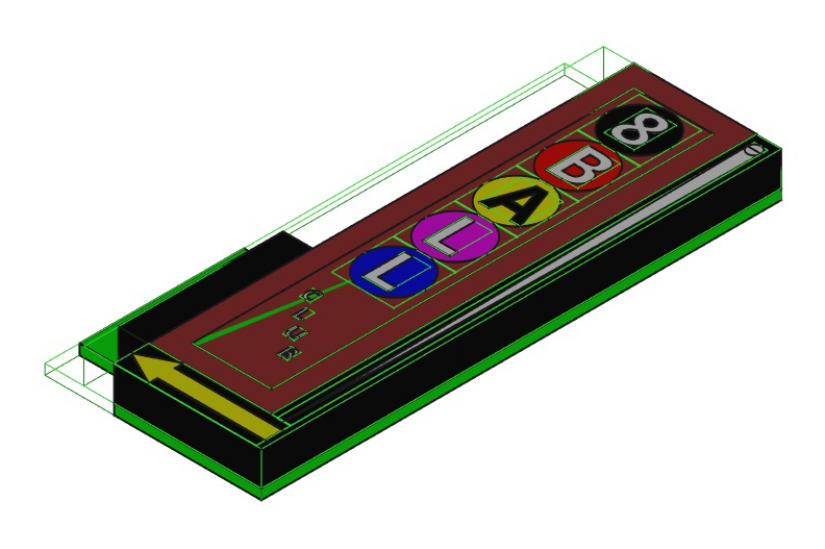
\includegraphics[height=2.5in]{8BallSign-ISOMetric.png}\\\end{centering}

This is a printed circuit board containing SMD LEDs meant to light a building 
side for a ``fictious'' pool hall, calling itself ``8 Ball Club''. The LEDs 
are arranged in five groups, each contain two sets of three LEDs in series 
with a current limiting resistor, one set on each side of the board.  It is 
meant to be powered from a 12V supply, which can be hard wired (very boring!) 
or under the control of a MCU (like an Arduino with a driver IC), that will 
light each of the five groups in sequence, that is like the flashy (trashy?) 
signs used for things like bars, dance halls, night clubs, and casinos. That 
is something to liven up either a seedy neighborhood or to add to a brightly 
lit ``strip''.

\begin{figure}[hbpt]\begin{centering}%
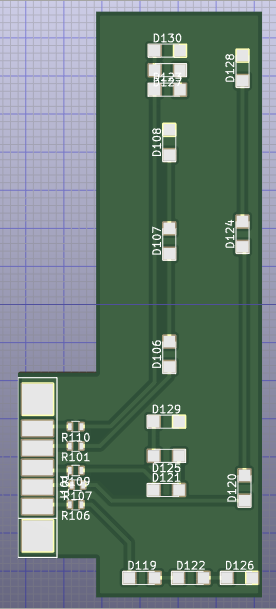
\includegraphics{8BallLEDPCB.png}
\caption{3D view of the board}
\end{centering}\end{figure}


\section{Assembly}
The PCB is meant to have printed artwork (typically printed with a color 
printer) and needs spacers to support the artwork above the LED chips. The 
spacers can be 3D printed.  The collection of files for both 3D (spacers) and 
2D (sign artwork) are available for download here: 
\url{https://www.thecountryrobot.com/wp-content/uploads/2023/11/8BallSignFiles.zip} \\

\includegraphics[height=1in]{8ballsign_qr_download.png}.

There are two spacers, one for each side. After 3D printing them,
\textbf{leave the skirt added by Cura on} and using Slow Zap (or other thick
CA glue), glue one side to the PCB. Once the glue has set, the skirt can be
trimmed off with a hobby knife. Repeat for the other side. You might want to
trim the skirt along the edge where the connection pads are before gluing
because the spacer is shorter that the PCB to expose the connection pads. The
spacers should made from a black or at least a dark colored filament.

Once the spacers are in place, cut the artwork from the printed sheet and also 
using Slow Zap, glue on the artwork.  Finally, the edges can be sanded smooth 
and painted black.

\section{Connecting the board}
\begin{figure}[hbpt]\begin{centering}%
\includegraphics{8BallLEDPCBContacts\_annotated.png}
\caption{Connection pad detail}
\end{centering}\end{figure}

The board has seven (7) through hole solder pads.  There are two ``commons'' 
-- these are wired together on the board and only one needs to be connected -- 
the two are provided for connection convenience. The common goes to the 
positive side of the supply and the other five connections connect to the 
negative side of the supply, one for each of the five groups.  The groups are 
meant to be lighted in order and cumulatively, starting with just the 8, then 
8 and BALL, then 8; BALL; and CLUB; then 8; BALL; CLUB; and the cue stick, 
then all of them, then all off, and repeat, but other patterns are certainly 
possible. 

To mount the sign cut a vertical slot in the building's face, typically at the 
second floor level over the main street entrance, to accommodate the wires and 
connection pads.  Feed the wires through this slot and seat the sign assembly 
and glue (with Slow ZAP) in place.

\end{document}
